\documentclass{report}
\usepackage[final]{pdfpages} %For using cover page pdf in the latex file
\usepackage[utf8]{inputenc}
\usepackage{geometry}
\usepackage{amsmath}
\usepackage{amsthm}
\usepackage{amsfonts}
\usepackage{amssymb}
\usepackage{graphicx}
\usepackage{tocloft}

%\usepackage{perpage} %the perpage package
%\MakePerPage{footnote} %the perpage package command

% For adding TOC in pdf bookmarks
\usepackage{hyperref}
\hypersetup{pdftex,colorlinks=true,allcolors=black}
\usepackage{hypcap}
%
\usepackage{float}
\usepackage{xepersian}
\usepackage{bidi}


\settextfont{Yas}
\SepMark{-}

\renewcommand{\cftsecleader}{\cftdotfill{\cftdotsep}}

\theoremstyle{definition}
\newtheorem{definition}{تعریف}

\title{طرح پیشنهادی پروژه کارشناسی}
\author{امیر حقیقتی ملکی}
\date{پاییز ۹۶}
	
\begin{document}
	%%%%%%%%%%%%%%%%%%%%%%%%%%%%%%%
	%%	 TITLE PAGE - BEGIN	     %%
	%%%%%%%%%%%%%%%%%%%%%%%%%%%%%%%
	\newgeometry{margin=1in}
	\pagenumbering{gobble}
	\begin{titlepage}
				\centering
		
\includegraphics[width=0.25\textwidth]{Resources/logo.png}\par\vspace{1cm}
		{\scshape\LARGE دانشگاه صنعتی امیرکبیر \par}
		{\scshape\LARGE دانشکده مهندسی کامپیوتر و فناوری اطلاعات \par}
		\vspace{1cm}
		{\scshape\Large
			بررسی طرح کلی پروژه کارشناسی
			\par}
		\vspace{1.5cm}
		{\huge\bfseries 
			پیاده‌سازی سامانه‌ای مبتنی بر وب برای سنجش کارایی رابط کاربری وب‌اپلیکیشن‌ها به روش جمع‌سپاری
			\par}
		\vspace{2cm}
		نگارنده:\par
		{\Large امیر حقیقتی ملکی\par}
		\href{mailto:amirh@aut.ac.ir}{amirh@aut.ac.ir}
		\vfill
		استاد راهنما:\par
		{\Large استاد احمد عبداله‌زاده بارفروش\par}
		\href{mailto:ahmad@ce.aut.ac.ir}{ahmad@ce.aut.ac.ir}
		\vfill
		
		% Bottom of the page
		{\large \rl{
				تابستان ۹۷
			}\par}
		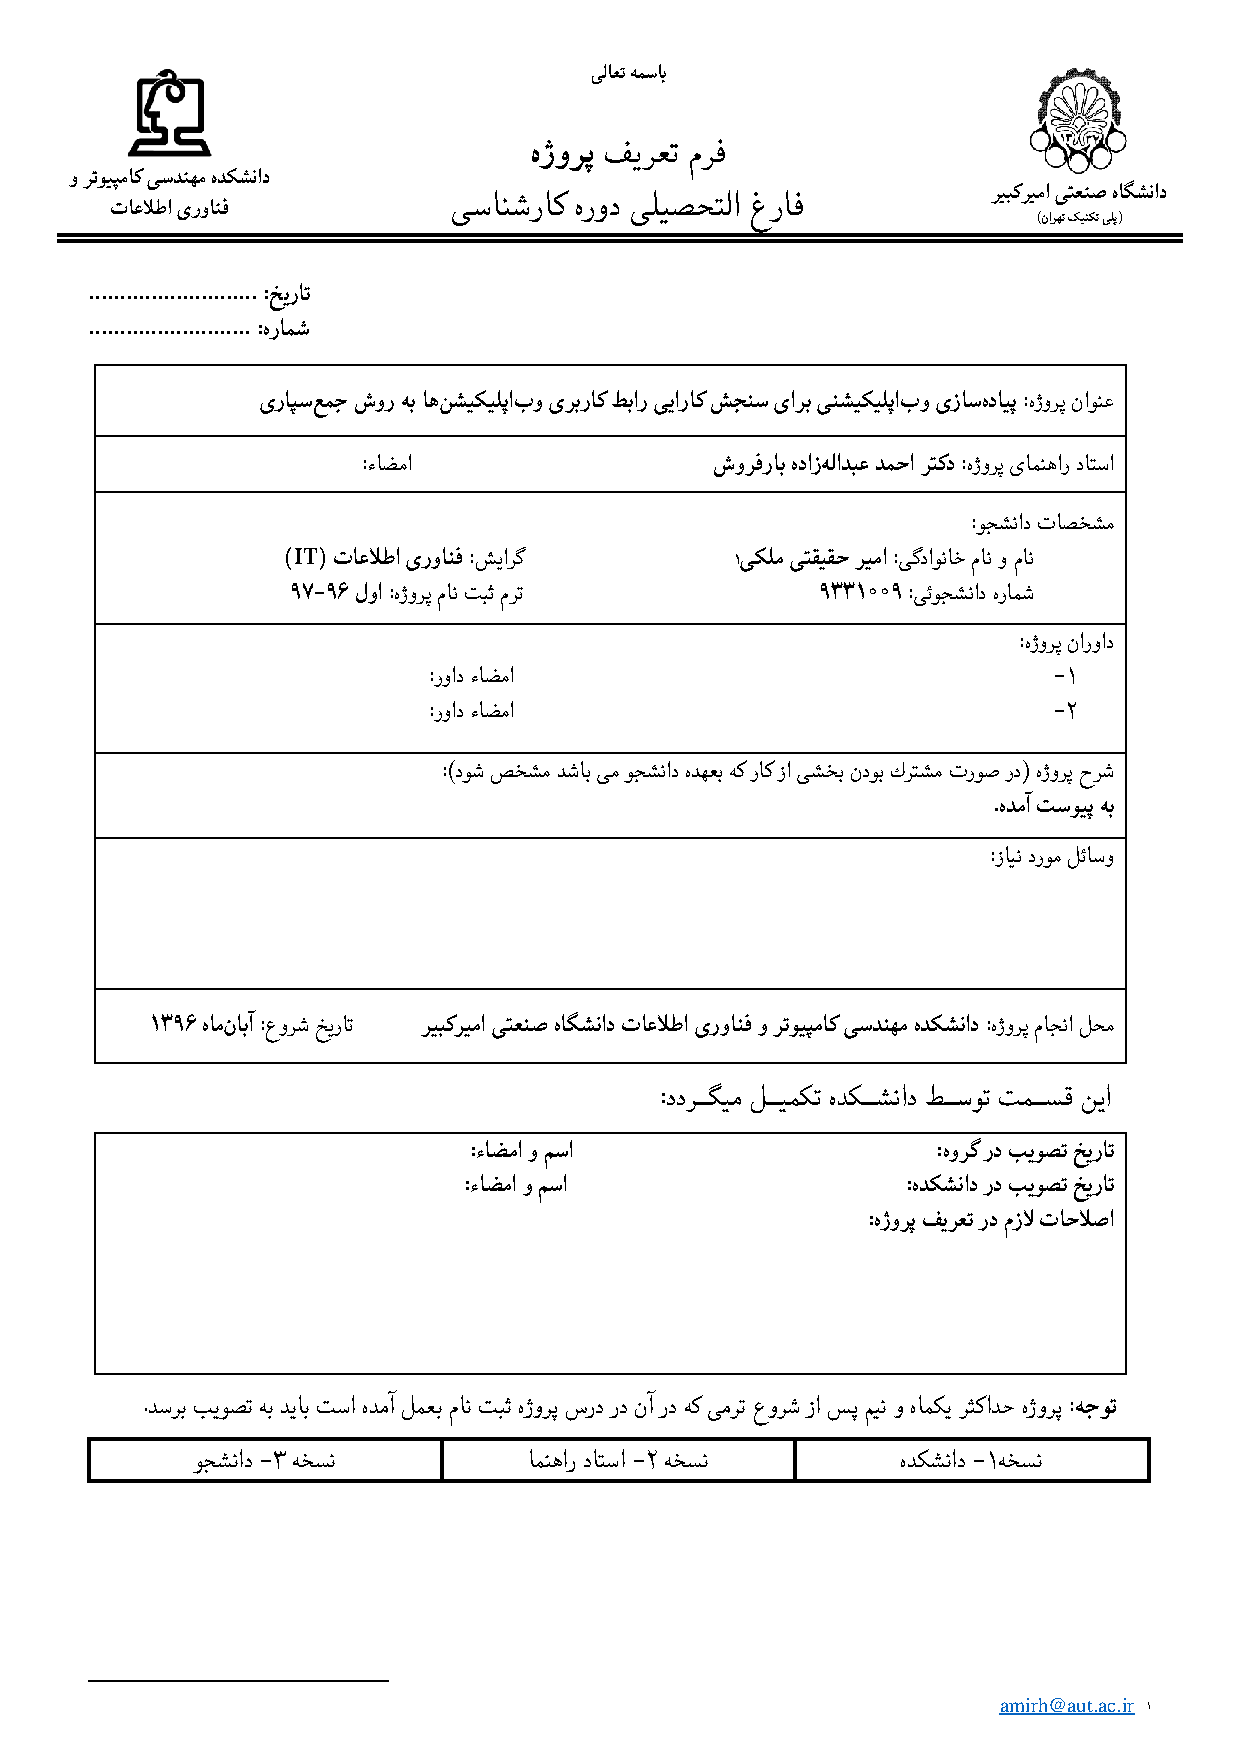
\includepdf[pages=-]{Project_Definition_Page.pdf}
	\end{titlepage}
	\newpage
	\pagenumbering{Alph}
	\begin{abstract}
		\thispagestyle{plain}
	با تقریب خوبی می‌توان گفت تمامی مدل‌های کیفی نرم‌افزار، کارایی را جزو مشخصه‌های اصلی کیفیت یک نرم‌افزار مطرح می‌کنند. وجه مشترک تعاریف متعددی که برای کارایی مطرح می‌شود، در سه بعد کاربر، انجام یک فعالیت مشخص و تعامل با یک واسط برای انجام آن فعالیت، قابل بیان است. به عنوان یک مهندس نرم‌افزار، افزایش کیفیت در محصولات و کاهش هزینه‌های ناشی از خرابی‌ها و یا درخواست‌های تغییر، چالشی تامل برانگیز است. وب‌اپلیکیشن‌ها به عنوان نوعی محصول نرم‌افزاری که در آن‌ها زیبایی، واسط کاربری و نحوه تعامل کاربران مهم است، به دلیل استفاده گسترده‌شان، می‌توانند تاثیر شگرفی در موفقیت یک پروژه صنعتی، کسب‌وکارهای نوپا و یا تسهیل زندگی روزمره با استفاده از نرم‌افزارها داشته باشند. از جمله نقاط ضعف بیشتر وب‌اپلیکیشن‌ها، طراحی نه‌چندان کاربرپسندانه واسط کاربری آن‌هاست که موجب شده تا در بسیاری از موارد، کاربران، علاقه‌مندی استفاده از محصول مبتنی وب یک سازمان را در عین سرمایه‌گذاری‌های زیاد آن سازمان برای جذب کاربر، از دست بدهند و در نتیجه متضرر شوند. گرچه، به صورت ایده‌آل، تمامی تصمیم‌گیری‌های مدیریتی و کلان (از قبیل اتخاذ مدل‌های فرایندی مناسب برای تولید نرم‌افزار با هزینه کم) با نهایت دقت و تجربه انجام می‌شوند، ولی در بسیاری از موارد همچون پروژه تقویم شرکت گوگل، مواردی ملاحظه می‌شود که واسط کاربری ناکارآمد، به ناچار، هزینه‌های گاهاً زیادی به تیم مهندسی نرم‌افزار تحمیل کرده است. با مروری بر منابع مختلف، ارزیابی و تست روی نمونه‌های اولیه رابط کاربری وب‌اپلیکیشن‌ها به منظور رفع نواقص آن‌ها، امری واضح به نظر می‌رسد. اما پاسخ دادن به این سوال که «چه واسط کاربری‌ای خوب است؟» همیشه آسان نبوده و با تغییر فناوری و گذشت زمان شاهد تغییر سریع در نیازمندی‌ها هستیم که شاید چک‌لیست‌ها و توصیه‌ها نیز پاسخگوی دقیقی برای آن‌ها نباشند. بنابراین می‌بایست در طراحی واسط کاربری، به یک روش کمی و قابل استناد، نیازمندی‌ها را با استفاده از نمونه‌های اولیه بسنجیم (که به دلیل هنری انگاشتن اکثر کارها، این امر نادیده گرفته می‌شود). اما سنجش دقیق، نیازمند جمع‌آوری داده از ارزیابی و تست واسط کاربری توسط کاربران نهایی است تا بتوان تحلیل دقیق انجام داد و مشکلات طراحی واسط را به درستی تشخیص داد. یکی از روش‌های جمع‌آوری داده، استفاده از جمع‌سپاری است. باید توجه داشت که استفاده از جمع‌سپاری چالش‌هایی را فرارویمان خواهد گذاشت که از جمله آن‌ها میتوان به عدم وجود صحت در داده‌ها اشاره کرد. در این پروژه وب‌اپلیکیشنی به منظور ارائه داشبورد مدیریتی برای صاحبان طراحی و افراد متمایل به انجام تست‌های مختلف با معیارهای متفاوت و دلخواه، پیاده خواهد شد. همچنین دادگان و پاسخ‌ها و تحلیل‌های تست اپلیکیشن در مواجهه کاربران واقعی با آن‌ها، به اطلاع کاربر خواهد رسید؛ علاوه بر موارد فوق، قسمت اصلی این پروژه در پاسخ به چالش صحت داده در روش جمع‌سپاری، ابتدا رفتار کاربران پاسخ‌دهنده (کارگران) توسط ماتریسی مدل می‌شود که برای مدل‌سازی و به دست آوردن مقادیر مدل‌ها، از روش تزریق سوالات طلایی استفاده خواهد شد. سپس در صورت پایین بودن کیفیت کار کارگران از حد مشخصی که در هنگام مدل‌سازی مشخص می‌شود، نتیجه کار آن‌ها به عنوان داده نامربوط شناخته شده و حذف می‌گردد. امکان تعریف تست‌های دلخواه و محدود نبودن به تست‌های از پیش تعریف شده تفاوت عمده ابزار کارا با سایر ابزارهای مشابه است؛ از جمله ابزارهای مطرح موفق در این حوزه، می‌توان به UsabilityHub، Optimizely و CrazyEgg اشاره کرد که همانطور که ذکر شد، در طی این پروژه، سعی بر برطرف‌سازی برخی از نواقص آن‌هاست.
	\end{abstract}
	\newpage
	\pagenumbering{gobble}
	\tableofcontents
	\newpage
	\pagenumbering{arabic}
	\chapter{تعریف مسئله}
صحبت راجع به اهمیت افزایش کیفیت نرم‌افزار، مدل کیفی و نحوه رسیدن به آن، متامدل(های) کیفیت و ورود به بحث کارایی.
	\section{کارایی}
به تعبیر نویسندگان مرجع [measuring] هر نفر می‌تواند برای خودش تعریفی از کارایی ارائه نماید. در اینجا به ارائه چند نمونه اصلی از تعریف کارایی می‌پردازیم.
تعریف سازمان بین‌المللی استانداردها (ایزو) ...
تعریف UPA...
تعریف کتاب Don’t Make Me Think...
بحث در مورد کارایی [measuring] و رابطه آن با تجربه کاربری ...
با بررسی مدل‌های کیفی مختلف که به منظور سنجش کمی کیفیت نرم‌افزار ارائه شده‌اند، مشاهده می‌شود که کارایی نرم‌افزار، به عنوان یکی از مشخصه‌های اصلی در اغلب این مدل‌ها به صورت صریح  بیان شده است. مدل‌های مک‌کال، Dromey، ایزو ۹۱۲۶، FURPS و ایزو ۲۵۰۱۰ از مدل‌های اساسی و مدل‌های برتوئا، گکوآمو، آلوارو و راواشد از جمله مدل‌های خاص منظوره‌ای هستند که در آن‌ها کارایی نرم‌افزارها به صورت صریح به عنوان یک فاکتور اصلی بیان شده است [بررسی مدل‌های کیفیت]. همچنین مفهوم کارایی نرم‌افزار به طور ضمنی در بطن اجزای سایر مدل‌های کیفی نهاده شده است. می‌توان گفت کارایی یک نرم‌افزار، از جمله ویژگی‌های مهم کیفی در دستیابی و کنترل کیفیت نرم‌افزار است.
	\section{تضمین و کنترل کیفیت}
همانطور که پرسمن در کتابش [پرسمن] مطرح می‌کند، رسیدن به یک محصول با کیفیت در مهندسی نرم‌افزار، به صورت ضمنی و خود به خود ممکن نیست؛ بلکه نتیجه بازنگری در چهار بعد کلی در فرآیند مهندسی نرم‌افزار و اِعمال مجموعه آن‌ها است: روش‌های مهندسی نرم‌افزار، تکنیک‌های مدیریت پروژه، فعالیت‌های کنترل و تضمین کیفیت نرم‌افزار. طبق این اظهار نظر، با فرض اِعمال شدن روش‌های درست و بهره‌ور مهندسی نرم‌افزار و تکنیک‌های موثر در مدیریت پروژه تولید نرم‌افزار - که با تقریب خوبی هر دو را می‌توان جزو روش‌های مدیریتی و در حوزه تصمیم‌گیری‌های کلان سیستم دانست - بدیهی است که همچنان کنترل کیفیت و تضمین آن، دو بعد فنی و جزئی‌تر رسیدن به نرم‌افزار با کیفیت را تشکیل می‌دهند. بنابراین می‌بایست روش‌های موثر به منظور انجام فرایند‌های کنترل کیفیت و تضمین رسیدن به آن، توسط تیم مهندسی نرم‌افزار اتخاذ شود.
اما، مشابه هر فرایند و فعالیت دیگری، رسیدن به کیفیت نیز هزینه‌های خاص خود را دارد. هزینه کیفیت در نرم‌افزار، مطابق اظهارنظر پرسمن، به سه دسته هزینه‌های پیش‌گیری، هزینه‌های ارزیابی و هزینه‌های خرابی تقسیم می‌شود[پرسمن]. هرکدام از این هزینه‌ها، در صورت پیش‌بینی و رفع نواقص محتمل/پیش‌آمده در هر مرحله از طراحی و پیاده‌سازی، بدون اینکه وارد مرحله بعدی شویم، می‌تواند به شدت کاهش یابد [پرسمن].
\subsection{رابط کاربری، کاهنده یا افزاینده کیفیت؟}
یکی از علل عدم رضایت کاربران و مشتریان از وب‌اپلیکیشن‌ها - که درنتیجه این نارضایتی، آمار کاربران وب‌اپلیکیشن‌های کسب‌وکارها دستخوش تغییرات نامطلوب شده و حتی هزینه‌های گزافی به تیم مهندسی نرم‌افزار به خاطر اعمال تغییر پس از تحویل، وارد می‌شود- طراحی نه‌چندان کاربرپسندانه واسط کاربری و زیبایی آن‌هاست [Assessing a Firm's]؛ بدیهی است که استفاده از مدل‌های فرایندی چابک می‌تواند در کاهش هزینه‌های طراحی مجدد پس از تحویل و یا اعمال تغییر در رابط کاربری موجود، موثر باشد [پرسمن]، اما هنوز یک سوال بدون پاسخ خواهد ماند: چه رابط کاربری‌ای برای کاربران وب‌اپلیکیشن (محصول) من مناسب است و طبق نیازمندی‌های فعلی حداکثر کیفیت را تامین خواهد کرد؟ برای پاسخ به این سوال چک‌لیست‌ها و توصیه‌های فراوانی [پرسمن و سامرویل] ارائه شده است که هرکدام به نحوی در افزایش کیفیت رابط‌های کاربری تاثیرگذار بوده‌اند [مقالات سروی]، اما برای تست یک رابط کاربری به صورت کمی، تحلیل و یافتن نقاط ضعف، به نظر می‌رسد که بررسی بیشتری مورد نیاز است.
\section{کارایی در طراحی رابط کاربری وب اپلیکیشن‌ها}
کارایی در وب‌اپلیکیشن‌ها - که امروزه نقش مهمی در ارائه محتوا و سرویس به کاربران دارند - به عنوان یکی از ابعاد و مشخصه‌های اصلی و مهم در کیفیت مطرح است [پرسمن]. یکی از عوامل بسیار تاثیرگذار در کارایی هر محصولی، رابط کاربری آن است، همچنین کیفیت و چگونگی طراحی رابط کاربری حتی می‌تواند به مرگ و زندگی افراد ختم شود [measuring]. پرواضح است که هرچه مشکلات و نواقص رابط‌های کاربری زودتر پیدا شده و مرتفع گردند، با پرداخت هزینه (تلاش و زمان) کمتر به کیفیت بیشتری رسیده‌ایم.
\subsection{چرخه طراحی واسط کاربری وب‌اپلیکیشن‌ها}
از جمله مراحل هرم طراحی وب‌اپلیکیشن [پرسمن]، طراحی واسط کاربری است. قبل از تولید کد وب‌اپلیکیشن، این واسط به صورت یک نمونه اولیه و در قالب طرح‌های ابتدایی، ماکت‌های مفهومی و یا چارچوب‌های کلی توصیف و طراحی می‌شوند. پس از رسیدن به توافق با مشتری (در صورت نیاز) و یا اعمال تغییرات متعدد تا رسیدن به توافق، این طراحی به کد قابل اجرا و پیاده‌سازی روی وب‌اپلیکیشن تبدیل می‌شود و نهایتا به تولید واسط کاربری آن می‌انجامد [رفرنس از توضیح روند طراحی].
...شکل مورد نیاز است…
مطابق آنچه در قسمت تضمین و کنترل کیفیت گفته شد، در صورت ارزیابی، تحلیل و رفع ایرادات مربوط به کارایی رابط کاربری، در همان مراحل ابتدایی و پس از تولید نمونه‌اولیه، می‌توان هزینه‌های بعدی را به طور قابل ملاحظه‌ای کمتر کرد.
مانند هر روش کیفی دیگری در تضمین کیفیت نرم‌افزار، به منظور دستیابی به کارایی قابل قبول (مطابق نیازهای مشتری) در واسط کاربری وب‌اپلیکیشن‌ها (همچون هر مشخصه اصلی دیگری) می‌بایست فاکتورها، معیارها و مولفه‌های مختلفی به منظور خرد و قابل اندازه‌گیری کردن این مفهوم کلان مطرح شود به طوری که بتوان در قالب مقادیر کمی، نیازمندی‌ها را با داده‌های به دست آمده از ارزیابی رابط کاربری وب‌اپلیکیشن مقایسه و تحلیل کرد. اما در بسیاری از موارد، همانطور که [منابع مختلف] ذکر می‌کنند، حقیقت محض و یا هیوریستیک تضمین‌کننده‌ای برای رسیدن به یک رابط کاربری «خوب» وجود ندارد و طراحی‌های کارا و موثر موفقیت خود را اغلب یا به روش‌های تجربی، که الزاماً با روش‌های علمی به اثبات نرسیده‌اند، و یا به ذوق هنری طراح مدیون‌اند [نیازمند منبع].
\section{جمع‌سپاری}
در سال ۲۰۱۲، با بررسی‌های مرجع [۶]، حدود ۴۰ تعریف مختلف در مقالات و پژوهش‌های علمی، حتی گاهی تعاریف متناقض با هم، برای جمع‌سپاری ارائه شده است. نویسندگان آن اثر، با درنظر گرفتن ابعاد مطرح در تعاریف مختلف، در نهایت تعریف نسبتا مفصلی از این مفهوم ارائه می‌دهند:
«باید ترجمه شود: 
جمع‌سپاری نوعی فعالیت برخط مشارکتی است که طی آن یک فرد، یا یک سازمان با ابزارهای کافی به گروهی از افراد با سطح دانش متغیر 
Crowdsourcing is a type of participative online activity in which an individual, organization, or company with enough means proposes to a group of individuals of varying knowledge, heterogeneity, and number, via a flexible open call, the voluntary undertaking of a task. The undertaking of the task, of variable complexity and modularity, and in which the crowd should participate bringing their work, money, knowledge and/or experience, always entails mutual benefit. The user will receive the satisfaction of a given type of need, be it economic, social recognition, self-esteem, or the development of individual skills, while the crowdsourcer will obtain and utilize to their advantage that what the user has brought to the venture, whose form will depend on the type of activity undertaken.
پایان ترجمه.»

شرح انگیزه‌های استفاده از جمع‌سپاری…
شرح چندی از کاربردهای جمع‌سپاری...
\subsection{جمع‌سپاری برای جمع‌آوری داده}
انگیزه اصلی استفاده از جمع‌سپاری و توضیح آن…
\chapter{جزییات فنی سیستم هدف و روش مورد استفاده}
\section{نمودار Use Case}
ساختار سیستم و اجزای آن که در شکل ۱ مشاهده می‌شود.

شکل ۱. نمودار Use Case سامانه کارا




\begin{thebibliography}{20}
	\begin{latin}
	\begin{LTRitems}
		\bibitem{main1} \lr{
			R. Pressman and B. Maxim, SOFTWARE ENGINEERING: A PRACTITIONER’S APPROACH, 8th ed. New York: McGraw-Hill Education, 2015.
		}
		\bibitem{main2} \lr{
			J. P. Miguel, D. Mauricio and G. Rodríguez, "A Review of Software Quality Models for the Evaluation of Software Products", International Journal of Software Engineering \& Applications, vol. 5, no. 6, pp. 31-53, 2014.
		}
		\bibitem{main3} \lr{
			R. Agarwal and V. Venkatesh, "Assessing a Firm's Web Presence: A Heuristic Evaluation Procedure for the Measurement of Usability", Information Systems Research, vol. 13, no. 2, pp. 168-186, 2002.
		}
		\bibitem{main3} \lr{
			T. Tullis and W. Albert, Measuring the user experience, 3rd ed. Amsterdam: Elsevier, 2013.
		}
		\bibitem{main4} \lr{
			E. Estellés-Arolas and F. González-Ladrón-de-Guevara, "Towards an integrated crowdsourcing definition", Journal of Information Science, vol. 38, no. 2, pp. 189-200, 2012.
		}
		\end{LTRitems}
	\end{latin}
\end{thebibliography}

	
\end{document}